\documentclass[border=6pt]{standalone}
\usepackage{amsmath}
\usepackage{tikz}
\usetikzlibrary{arrows.meta}
\begin{document}
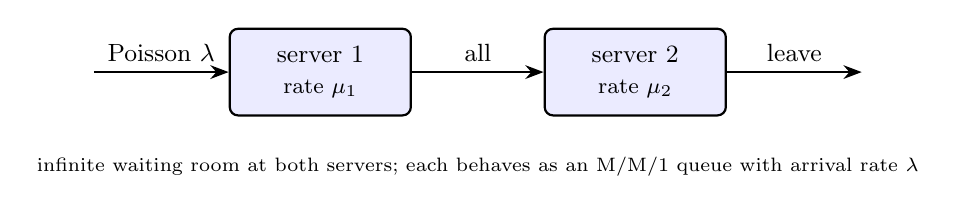
\begin{tikzpicture}[>=Stealth,font=\small,
 s/.style={draw,thick,circle,minimum size=1.1cm,inner sep=0pt,fill=blue!8},
 e/.style={->,thick},
 lab/.style={font=\small,fill=white,inner sep=1.5pt},
 every loop/.style={->,thick,looseness=6}]
\tikzset{st/.style={draw,thick,rounded corners=3pt,fill=blue!8,align=center,minimum width=2.3cm,minimum height=1.1cm}}
\node (in) at (0,0) {};
\node[st] (1) at (3,0) {server 1\\{\footnotesize rate $\mu_1$}};
\node[st] (2) at (7,0) {server 2\\{\footnotesize rate $\mu_2$}};
\node (out) at (10,0) {};
\draw[e] (in) -- node[above]{Poisson $\lambda$} (1);
\draw[e] (1) -- node[above]{all} (2);
\draw[e] (2) -- node[above]{leave} (out);
\node[font=\scriptsize,align=center] at (5,-1.2) {infinite waiting room at both servers; each behaves as an M/M/1 queue with arrival rate $\lambda$};
\end{tikzpicture}
\end{document}
